% !TeX root = ../thesis.tex

\chapter{Fundamentals}
\label{sec:fundamentals}

This chapter is dedicated to highlighting pre-requisite knowledge in machine learning needed for understanding the contribution and contents of the presented work.
%If not indicated otherwise, fundamentals of neural networks are taken from [blablabla]

\section{Artificial Neural Networks}

\gls{anns}, also commonly referred to as \textit{neural networks} are considered to  be universal function approximators \cite{Hornik1989}. ANNs are machine learning models that are inspired by human brain's biological neural network. A neuron is fundamental computational unit of human brain that is responsible for receiving sensory input via dendrites, process and generate output through axons, see \ref{fig: neuron}. Neurons are therefore the building blocks of brain's inter-connected neural network that processes and transmits information in the form of electrochemical signals. 


\begin{figure}[!htb]
	 \centering 
\includegraphics[scale = 0.35]{Graphics/Fundamentals/neuron3x} 
	\caption{Diagram of a biological neuron \cite{RTS20}} 
	\label{fig: neuron} 
\end{figure}

%Although artificial neural networks attempt to simulate characteristics of a biological neural network, state-of-the-art ANNs have never achieved full functional complexity and computational efficiency of their biological counterparts. 


\subsection{Multi-Layer Perceptron}


In 1943, McCulloch and Pitts tried to understand how brain could produce highly complex patterns by using many basic cells that are connected together and presented a simple model \cite{Arbib2004}. In 1958, Frank Rosenblatt proposed a generalized variant of a former, more simple structure to model brain activities by using single layer network \cite{Rosenblatt1958}. 



\begin{figure}[!ht]
	 \centering 
\includegraphics[scale = 0.2]{Graphics/Fundamentals/perceptron1} 
	\caption[Mathematical model of a Perceptron]{Mathematical model of a perceptron. Elements $x_i$ of an input \textbf{x} are multiplied individually with learnable weights $w_i$ and aggregated with an additional learnable bias term. The resultant is processed by a following non-linear activation function $f(.)$ to generate output. \cite{CS231n} }
	\label{fig: perceptron} 
\end{figure}
Structurally, perceptron attempts to replicate the basic phenomenon of receiving multiple input signals and processing them using learnable weights to generate an output.  A perceptron is able to learn weights depending on input-output correspondences, it therefore enables perceptrons to classify information.
As illustrated in \ref{fig: perceptron}, incoming input elements of \textbf{x} are multiplied with corresponding learned weights \textbf{w} (equivalent to a dot product between vectors \textbf{x} and \textbf{w}). Result is then added with another learnable input-independent bias term \textit{b}. 


\begin{equation}a_{\mathbf{x}}=\sum_{i=0} w_{i} x_{i}+b\end{equation}

Final output is generated by passing this weighted sum through a non-linear activation function $f(.)$ which will be explained in a later section in more detail:

%\begin{equation}{\textit{output}}= f\left(\sum_{i} w_{i} x_{i}+b\right)\end{equation}
\begin{equation}{\mathrm{output}}= f\left(\sum_{i=0} w_{i} x_{i}+b\right)\end{equation}


Multiple perceptrons when stacked above each other result in a \textit{layer}, while each perceptron in a layer is referred to as a \textit{node}. Nodes when connected to the nodes of a successive layer in a sequential structure, represent a \gls{mlp}, also known as a \textit{feed-forward neural network} \cite{Svozil1997}. see figure \ref{fig:mlp}.
Number of nodes in a hidden layer define \textit{width} of a network, while model's \textit{depth} is specified by the number of layers chained sequentially to form a neural network structure.

Such a feed forward neural network is used to learn data with multiple features, indicated by  number of input units. Each feature contributes to the output i.e, features are processed independently and information is carried out to the subsequent layers. Node in each layer receives inputs from nodes of preceding layer, processes them by calculating sum of product of each input with corresponding weights and passes the resultant through a non-linear activation function before forwarding to the nodes of following layer. 

Multi-layer structure is an essential modelling feature and furnishes prime contribution. MLP is assumed to learn discriminative features in a hierarchical manner \cite{Goodfellow-et-al-2016}. Lower layers in a network usually learn low-level features, while higher layers build upon these low-level features to generate higher level features. For instance, in digit classification problem, initial layers might discriminate between the presence of straight lines or curves, while higher layers might learn the structural correspondences among theses shapes to discriminate digits. Therefore, it can be loosely compared to a decision tree, where decision for the next stage is based on existence or non-existence of learned features and ultimately final result is built up respecting the features in preceding stages.

\begin{figure}[!ht]
	 \centering 
    %        \includegraphics[scale = 0.30]{Graphics/Fundamentals/mlp_latex}
        \begin{neuralnetwork}[height=5]
            \newcommand{\x}[2]{$x_#2$}
            \newcommand{\y}[2]{$\hat{y}_#2$}
            \newcommand{\hfirst}[2]{\small $h^{(1)}_#2$}
            \newcommand{\hsecond}[2]{\small $h^{(2)}_#2$}
            \inputlayer[count=3, bias=true, title=Input\\layer, text=\x]
            \hiddenlayer[count=4, bias=false, title=Hidden\\layer 1, text=\hfirst] \linklayers
            \hiddenlayer[count=3, bias=false, title=Hidden\\layer 2, text=\hsecond] \linklayers
            \outputlayer[count=2, title=Output\\layer, text=\y] \linklayers
        \end{neuralnetwork}
	\caption[Multi-Layer Perceptron]{Feed forward neural network graph of 3-layer perceptron with 3 input units and a bias term $x_0$, 2 hidden layers and 2 output nodes.The $1^{st}$ and $2^{nd}$ hidden layers contains 4 and 3 hidden units (nodes), respectively \cite{MULTILAYERPERCEPTRON}. }
	\label{fig:mlp} 
\end{figure}


\subsection{Activation Functions}

Activation function is a key component of a neural network since it adds non-linearity in the model. In a perceptron, the weighted sum is a linear combination of the input values. In order to model non-linear functions, it is necessary to allow for non-linearities within the network. Without a non-linearity, network with multiple hidden layers would collapse to network with a single hidden layer. Therefore, the weighted sum is passed through an activation function $f(.)$ before advancing it to a successive layer. Some of the most popular activation functions are \textit{sigmoid function}, \textit{hyperbolic tanget}, \textit{rectified linear or ReLU} and \textit{Leaky ReLU}, see figure \ref{fig:Activation functions}. ReLU - as described by the equation \ref{eq:ReLu}, is however most commonly recommended activation function for deep neural networks since rectifying neurons make for an even better model of biological neurons and yield equal or better performance than hyperbolic tangent and logistic sigmoid activation function based networks \cite{Glorot2011}. 
\begin{equation}f(x)=\left\{\begin{array}{ll}
x & \text { if } x \geq 0 \\
0 & \text { otherwise }
\end{array}\right.
\label{eq:ReLu}
\end{equation}

Compared to \textit{sigmoid or tanh} functions, it has been found to greatly accelerate the convergence of \gls{sgd} \cite{Krizhevsky2017} and does not contain complex computations such as exponential unlike its counterparts.
However, ReLU units are fragile and can “die” due to large gradient flowing through a ReLU neuron could cause the weights to update in such a way that the neuron will never activate again. Leaky ReLUs attempt to fix the aforementioned problem of ``dying ReLU" by having a small negative slope about $0.01$ insted of zero in regime $(x<0)$, see equation \ref{eq:LeakyReLu} \cite{CS231n}.
\begin{equation}f(x)=\left\{\begin{array}{ll}
0.01 & \text { for } x<0 \\
1 & \text { for } x \geq 0
\end{array}\right.
\label{eq:LeakyReLu}
\end{equation}

\begin{figure}[!ht]
%\centering
    \subfigure[sigmoid function]{
        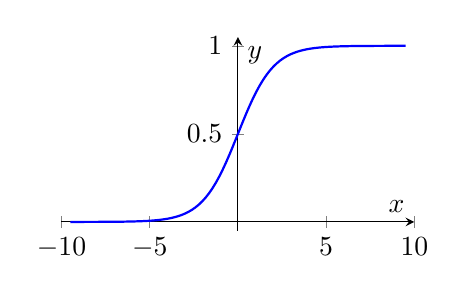
\begin{tikzpicture}
            \begin{axis}[
                axis lines=middle,
                xmax=10,
                xmin=-10,
                ymin=-0.05,
                ymax=1.05,
                xlabel={$x$},
                ylabel={$y$}, width = \textwidth /2, height = \textwidth / 3
            ]
            \addplot [domain=-9.5:9.5, samples=100,
                      thick, blue] {1/(1+exp(-x)};
            \end{axis}
        \end{tikzpicture}
    \label{fig:sigmoid}}
    \hfill
     %add desired spacing between images, e. g. ~, \quad, \qquad, \hfill etc.
     %(or a blank line to force the subfigure onto a new line)
    \subfigure[tanh function]{
       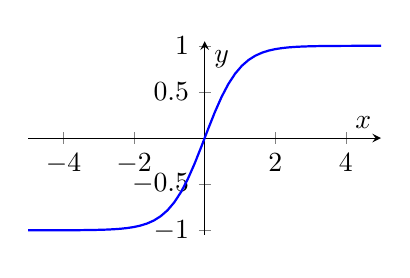
\begin{tikzpicture}
            \begin{axis}[
                axis lines=middle,
                xmax=5,
                xmin=-5,
                ymin=-1.05,
                ymax=1.05,
                xlabel={$x$},
                ylabel={$y$}, width = \textwidth /2, height = \textwidth / 3]
            \addplot [domain=-9.5:9.5, samples=100,
                 thick, blue] {(exp(x) - exp(-x))/(exp(x) + exp(-x))};
            \end{axis}
        \end{tikzpicture}
    \label{fig:tanh}}
    %\hspace{10pt}
    \subfigure[ReLU]{
        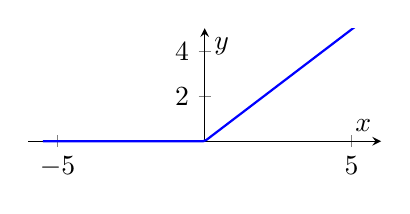
\begin{tikzpicture}
            \begin{axis}[
                axis lines=middle,
                xmax=6,
                xmin=-6,
                ymin=-0.05,
                ymax=5.05,
                xlabel={$x$},
                ylabel={$y$}, width = \textwidth /2, height = \textwidth / 4]
            \addplot [domain=-5.5:5.5, samples=100, thick, blue] {max(0, x)};
            \end{axis}
        \end{tikzpicture}
    \label{fig:ReLU}}
    \hfill
    \subfigure[Leaky ReLU]{
        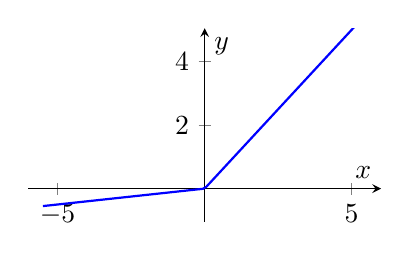
\begin{tikzpicture}
            \begin{axis}[
                axis lines=middle,
                xmax=6,
                xmin=-6,
                ymin=-1.05,
                ymax=5.05,
                xlabel={$x$},
                ylabel={$y$},  width = \textwidth /2, height = \textwidth / 3]
            \addplot [domain=-5.5:5.5, samples=100,
                  thick, blue] {max(0.1 * x, x)};
        \end{axis}
    \end{tikzpicture}
    \label{fig:Leaky ReLU}}
    \caption[Characteristic curves for activation functions]{Characteristic curves for Activation Functions a) sigmoid - $output=\frac{1}{1+e^{-x}}$  b) hyperbolic tanget - $output=\frac{e^{x}-e^{-x}}{e^{x}+e^{-x}}$ c) rectified linear (ReLU) - $output=\max (0, x)$  d) Leaky ReLU - $output=\max (0.01 \times x, x)$ \cite{FUNCTIONS}}
    \label{fig:Activation functions}
\end{figure}


\subsection{Optimization}
\label{subsec:learningnopt}
This section is dedicated to brief description of the learning process within a neural network.
In supervised learning, network learns from multiple sets of input-groundtruth $($\textbf{x}$, y_{gt})$ pairs commonly known as \textit{training set} in an iterative process. To this end, backpropogation method is employed to update the weights \textbf{w} \textit{(learning)} according to a performance measure of network in each step.

When an input \textbf{x} is fed into such a \textit{feed-forward neural network}, it sequentially multiplies input elements $x_i$ with corresponding randomly initialised weights \textbf{w} until the \textit{output layer}, which generates the final predicted output $\hat{y}$. This output is then compared against the corresponding groudtruth label, objective is to update the network parameters $\mathbf{w}$ according to how ``incorrect" network was in its prediction. A common comparison criterion is \textit{Mean Squared Error} (MSE) - which as the name suggest is the mean of squared difference between the predicted $\hat{y}$ and groundtruth value $ y_{gt}$. Mathematically, it can be written as:
\begin{equation}L\left(\mathbf{w}, \mathbf{x}, \mathbf{y}_{\mathbf{gt}}\right)=\frac{1}{N} \sum_{\mathbf{i}}^{N}\left(\hat{y}_{i}(\mathbf{w}, \mathbf{x})-y_{gt, i}\right)^{2}\label{eq:mse}
\end{equation}

%Since, it is a common practice to find the loss for a certain subset of training set instead of every single sample %independently. Equation \ref{eq:mse} corresponds to MSE of a subset. 
The loss \textit{L} is low if the prediction is similar to the groundtruth value, and higher if dissimilar. The goal is then to minimize this \textit{loss function L} which in this case is, MSE based.
To minimize this loss, each parameter of $\mathbf{w}$ of the hidden layers of
the neural network is tuned such that it aids in lowering the overall difference between predicted and corresponding groundtruth values. \textit{Objective function} for minimising the loss then can be written as : 

\begin{equation}
\min _{\mathbf{w}} L\left(\mathbf{w}, \mathbf{x}, \mathbf{{y}_{\mathbf{gt}}}\right)
\end{equation}

This can be achieved by calculating the gradient of loss with respect to parameters and changing the current weights $\mathbf{w_{t}}$ such that the new weights $\mathbf{w_{t + 1}}$ result in minimum loss. Essentially, it is intended to select the weights in descent direction of the gradient:

\begin{equation}
- \frac{\delta}{\delta \mathbf{w}} L\left(\mathbf{w}, \mathbf{x}, \mathbf{y}_{\mathbf{gt}}\right)
\end{equation}

Since, the loss depends upon all the weights $\mathbf{w}$ and biases $\mathbf{b}$ in all hidden layers, it is important to calculate gradients with respect to all trainable dependent variables normally calculated using \textit{backpropagation algorithm} \cite{Svozil1997} which exploits chain-rule :
\begin{equation}\frac{d y}{d x}=\frac{d y}{d u} \frac{d u}{d x}\end{equation}

The derivatives for all the variables is calculated using back-propagation  algorithm by recursive application of chain-rule, the weights are then updated \textit{(learning)} using commonly employed \gls{gd} \cite{Goodfellow-et-al-2016}:

\begin{equation}\mathbf{w}_{\mathbf{t}_{\mathbf{i}+1}}=\mathbf{w}_{\mathbf{t}}-\gamma_{t_{i}} \frac{\delta}{\delta \mathbf{w}_{\mathbf{t}_{\mathbf{i}}}} L\left(\mathbf{w}_{\mathbf{t}_{\mathbf{i}}}, \mathbf{x}_{\mathbf{t}_{\mathbf{i}}}, \mathbf{y}_{\mathbf{g} \mathbf{t}, \mathbf{t}_{\mathbf{i}}}\right)\end{equation}


$\gamma_{t_{i}}$ is the \textit{learning rate} which represents how fast the network weights are adapted with respect to gradient.

\gls{sgd} is an incremental version of vanilla \gls{gd} which uses a subset of training set at each step instead of whole trainig set which has the benefit of faster convergence and generalization \cite{Rumelhart1986}. \textit{Adam}, is another commonly used optimizer which uses adaptive learning rate and has the advantage of better convergence due to adaptive nature \cite{Goodfellow-et-al-2016}. In the presented work, Adam has been employed as an optimizer during trainings.

\section{Convolutional Neural Network}

It can be observed that for larger dimensional inputs a classical artificial neural network \gls{anns} explodes in term of memory requirements. Consider an image with $200\times200$ spatial resolution and an ANN with $10$ \textit{nodes} in the first layer, the parameters end up being $200000$ for this layer only. Memory requirement is a problem but also the local co-relations are not taken into account, instead all the pixels are equally co-related leading to a lot of redundancy, slow optimisation and inference times. \textit{Convolutional Neural Networks} (CNNs), therefore are variant of ANNs that are well-suited for grid-like structured and spatially co-related data. 
\bigskip

\begin{figure}[!ht]
	 \centering 
        \includegraphics[scale = 0.7]{Graphics/Fundamentals/CNN.png} 
	\caption[Convolutional Neural Network]{Visualisation of a convolutional neural network with $5$ hidden layers}
	\label{fig: CNN} 
\end{figure}

\subsection{Convolution Operator}
Convolutional Neural Networks (\gls{cnns}) make use of \textit{convolution operator}. Convolution operations alleviate the problem of redundancy by re-using the same kernel over spatial dimensions and also model local co-relations across pixels. Since, \gls{cnns} respect the local spatial co-relations and are also memory efficient due to weight sharing properties. Therefore, CNNs are widely used for learning image based data for computer vision applications.

Convolution is an operation on two functions \textit{I} and \textit{K}, which produces a third function that can be interpreted as a filtered (``convolved") version of \textit{I}. \cite{SpatialConv}

\begin{equation}I[x, y] * K[x, y]=\sum_{m=-\infty}^{\infty} \sum_{n=-\infty}^{\infty} I\left[m, n\right] \cdot K\left[x-m, y-n\right]\end{equation}

Visualisation of such a 2D- convolution between an image and a kernel of size $3\times3$ can be seen in the figure \ref{fig:Conv} where a filter is applied across spatial dimension of the image to generate a filtered version of input image.


\begin{figure}[!ht]
	 \centering 
    %        \includegraphics[scale = 0.30]{Graphics/Fundamentals/mlp_latex}
        \begin{tikzpicture}

        	\matrix (mtr) [matrix of nodes,row sep=-\pgflinewidth, nodes={draw}]
        	{
        		0 & 1 & 1 & |[fill=red!30]| 1 & |[fill=red!30]| 0 & |[fill=red!30]| 0 & 0\\
        		0 & 0 & 1 & |[fill=red!30]| 1 & |[fill=red!30]| 1 & |[fill=red!30]| 0 & 0\\
        		0 & 0 & 0 & |[fill=red!30]| 1 & |[fill=red!30]| 1 & |[fill=red!30]| 1 & 0\\
        		0 & 0 & 0 & 1 & 1 & 0 & 0\\
        		0 & 0 & 1 & 1 & 0 & 0 & 0\\
        		0 & 1 & 1 & 0 & 0 & 0 & 0\\
        		1 & 1 & 0 & 0 & 0 & 0 & 0\\
        	};
        
        	\draw[very thick, red] (mtr-1-4.north west) rectangle (mtr-3-6.south east);
        
        	\node [below= of mtr-5-4.south] (lm) {$\mathbf{I} $};
        
        	\node[right = 0.2em of mtr] (str) {$*$};
        
        	\matrix (K) [right=0.2em of str,matrix of nodes,row sep=-\pgflinewidth, nodes={draw, fill=blue!30}]
        	{
        		1 & 0 & 1 \\
        		0 & 1 & 0 \\
        		1 & 0 & 1 \\
        	};
        	\node [below = of K-3-2.south] (lk) {$\mathbf{K} $};
        
        	\node [right = 0.2em of K] (eq) {$=$};
        
        	\matrix (ret) [right=0.2em of eq,matrix of nodes,row sep=-\pgflinewidth, nodes={draw}]
        	{
        		1 & 4 & 3 & |[fill=green!30]| 4 & 1\\
        		1 & 2 & 4 & 3 & 3\\
        		1 & 2 & 3 & 4 & 1\\
        		1 & 3 & 3 & 1 & 1\\
        		3 & 3 & 1 & 1 & 0\\
        	};
        	\node [below = of ret-4-3.south] (lim) {${\mathbf{I} } * {\mathbf{K} }$};
        
        	\draw[very thick, green] (ret-1-4.north west) rectangle (ret-1-4.south east);
        
        	\draw[densely dotted, blue, thick] (mtr-1-4.north west) -- (K-1-1.north west);
        	\draw[densely dotted, blue, thick] (mtr-3-4.south west) -- (K-3-1.south west);
        	\draw[densely dotted, blue, thick] (mtr-1-6.north east) -- (K-1-3.north east);
        	\draw[densely dotted, blue, thick] (mtr-3-6.south east) -- (K-3-3.south east);
        
        	\draw[densely dotted, green, thick] (ret-1-4.north west) -- (K-1-1.north west);
        	\draw[densely dotted, green, thick] (ret-1-4.south west) -- (K-3-1.south west);
        	\draw[densely dotted, green, thick] (ret-1-4.north east) -- (K-1-3.north east);
        	\draw[densely dotted, green, thick] (ret-1-4.south east) -- (K-3-3.south east);
        
        	\matrix (K) [right=0.2em of str,matrix of nodes,row sep=-\pgflinewidth, nodes={draw, fill=blue!10}]
        	{
        		1 & 0 & 1 \\
        		0 & 1 & 0 \\
        		1 & 0 & 1 \\
        	};
        
        	\draw[very thick, blue] (K-1-1.north west) rectangle (K-3-3.south east);
        
        	\node[anchor=south east, inner sep=0.01em, blue] at (mtr-1-4.south east) (xx) {\scalebox{.5}{$\times 1$}};
        	\node[anchor=south east, inner sep=0.01em, blue] at (mtr-1-5.south east) (xx) {\scalebox{.5}{$\times 0$}};
        	\node[anchor=south east, inner sep=0.01em, blue] at (mtr-1-6.south east) (xx) {\scalebox{.5}{$\times 1$}};
        	\node[anchor=south east, inner sep=0.01em, blue] at (mtr-2-4.south east) (xx) {\scalebox{.5}{$\times 0$}};
        	\node[anchor=south east, inner sep=0.01em, blue] at (mtr-2-5.south east) (xx) {\scalebox{.5}{$\times 1$}};
        	\node[anchor=south east, inner sep=0.01em, blue] at (mtr-2-6.south east) (xx) {\scalebox{.5}{$\times 0$}};
        	\node[anchor=south east, inner sep=0.01em, blue] at (mtr-3-4.south east) (xx) {\scalebox{.5}{$\times 1$}};
        	\node[anchor=south east, inner sep=0.01em, blue] at (mtr-3-5.south east) (xx) {\scalebox{.5}{$\times 0$}};
        	\node[anchor=south east, inner sep=0.01em, blue] at (mtr-3-6.south east) (xx) {\scalebox{.5}{$\times 1$}};

        \end{tikzpicture}

	\caption[Visualisation of 2D Convolution Operation]{Visualisation of a 2D-convolution operation between Image \textit{I} and $3\times3$ kernel \textit{K} where \textit{I * K} represents the result after operation. \cite{MATCONV} }
	\label{fig:Conv} 
\end{figure}

It can also be seen from the figure \ref{fig:Conv} that spatial resolution of output is smaller than the input due to nature of convolution operation which results in reduced features in output. To remedy this effect, input is padded across the borders with extra 0s. Additionally, non-linearity such as ReLU as mentioned in \ref{eq:ReLu} is employed after convolution operations to avoid network from collapsing to a linear model. Therefore, each layer in a CNN has following parameters:

\begin{itemize}
    \item Number of filter kernels - N
    \item Spatial resolution of kernel - K
    \item Number of pixels, filter strides between two applications - S
    \item Number of zeros padded around the borders - P
\end{itemize}

Given the parameters, output dimensions of a convolutional layer in a CNN can be calculated as follows:

\begin{equation} H_{\text {output}}=\frac{H_{\text {input}}-K+2 P}{S}+1\label{eq:hout}\end{equation}
\begin{equation} W_{\text {output}}=\frac{W_{\text {input}}-K+2 P}{S}+1\label{eq:wout}\end{equation}
\begin{equation}D_{\text {output}}=N\label{eq:dout}\end{equation}

In the equations \ref{eq:hout} - \ref{eq:dout}, $H_{output}$, $W_{output}$ and $D_{output}$ correspond to height, width and depth size of the output from convolutional layer.


\subsection{Pooling Operator}

\label{subsec: pooling_operation}

From figure \ref{fig:Conv}, it can be seen that the depth of output is usually increased relative to the input which leads to an increase in the values calculated during the forward pass, even modern Graphics Processing Units (GPUs) might not be able to hold them in memory specially if the \gls{cnns} is very deep - has large number of layers. To avoid this computational expense, pooling operations are used to reduce the spatial dimensions of calculated feature outputs while keeping necessary information.

Pooling operation also helps in improving generalization by considering translational in-variances of features calculated in a convolutional layer.

Pooling is a spatial down-sampling operation with two variations:

\begin{itemize}
    \item Max-pooling  - from a spatial window of $K$ x $K$, maximum value is picked
    \item Average-pooling - from a spatial window of $K$ x $K$, average value is calculated 
\end{itemize}


 \begin{figure}[!ht]
	 \centering 
        \begin{tikzpicture}
            \fill [c1] (0, 0) rectangle (2, 2);
            \fill [c2]   (2, 0) rectangle (4, 2);
            \fill [c3]  (4, 0) rectangle (6, 2);
            \fill [c4] (0, 2) rectangle (2, 4);
            \fill [c5]   (2, 2) rectangle (4, 4);
            \fill [c6]   (4, 2) rectangle (6, 4);
        
            \fill [c1]  (9.5, 1) rectangle (10.5, 2);
            \fill [c2]   (10.5, 1) rectangle (11.5, 2);
            \fill [c3]  (11.5, 1) rectangle (12.5, 2);
            \fill [c4]  (9.5, 2) rectangle (10.5, 3);
            \fill [c5]   (10.5, 2) rectangle (11.5, 3);
            \fill [c6]   (11.5, 2) rectangle (12.5, 3);
        
            \foreach \i in {\xMin,...,\xMax} {
                \draw [very thin,gray] (\i,\yMin) -- (\i,\yMax)  node [below] at (\i,\yMin) {};
            }
            \foreach \i in {\yMin,...,\yMax} {
                \draw [very thin,gray] (\xMin,\i) -- (\xMax,\i) node [left] at (\xMin,\i) {};
            }
        
            \foreach \i in {\xMin,2,...,\xMax} {
                \draw [thick,gray] (\i,\yMin) -- (\i,\yMax)  node [below] at (\i,\yMin) {};
            }
            \foreach \i in {\yMin,2,...,\yMax} {
                \draw [thick,gray] (\xMin,\i) -- (\xMax,\i) node [left] at (\xMin,\i) {};
            }
            \node at (0.5, 0.5) {7};
            \node at (1.5, 0.5) {9};
            \node at (2.5, 0.5) {3};
            \node at (3.5, 0.5) {5};
            \node at (4.5, 0.5) {9};
            \node at (5.5, 0.5) {4};
            %
            \node at (0.5, 1.5) {0};
            \node at (1.5, 1.5) {7};
            \node at (2.5, 1.5) {0};
            \node at (3.5, 1.5) {0};
            \node at (4.5, 1.5) {9};
            \node at (5.5, 1.5) {0};
            %
            \node at (0.5, 2.5) {5};
            \node at (1.5, 2.5) {0};
            \node at (2.5, 2.5) {9};
            \node at (3.5, 2.5) {3};
            \node at (4.5, 2.5) {7};
            \node at (5.5, 2.5) {5};
            %
            \node at (0.5, 3.5) {9};
            \node at (1.5, 3.5) {2};
            \node at (2.5, 3.5) {9};
            \node at (3.5, 3.5) {6};
            \node at (4.5, 3.5) {4};
            \node at (5.5, 3.5) {3};
        
            \draw[draw=black,line width=12pt,-{Latex[length=9mm]}] (6.5, 2)  -- (9,2);
            \node[font=\footnotesize\bfseries] at (7.7, 2.5) {$\mathbf{2\times 2}$ max pooling};
        
            \foreach \i in {\xMinR,...,\xMaxR} {
                \draw [thick,gray] (\i,\yMinR) -- (\i,\yMaxR)  node [below] at (\i,\yMinR) {};
            }
            \foreach \i in {\yMinR,...,\yMaxR} {
                \draw [thick,gray] (\xMinR,\i) -- (\xMaxR,\i) node [left] at (\xMinR,\i) {};
            }
        
            \node at (10, 1.5) {9};
            \node at (11, 1.5) {5};
            \node at (12, 1.5) {9};
            \node at (10, 2.5) {9};
            \node at (11, 2.5) {9};
            \node at (12, 2.5) {7};
        
            \draw [decorate,decoration={brace,amplitude=4pt},xshift=-2pt,yshift=0pt]
        (0,2) -- (0,4) node [black,midway,xshift=-0.3cm] {\footnotesize $2$};
        
            \draw [decorate,decoration={brace,amplitude=4pt},xshift=0pt,yshift=2pt]
        (0,4) -- (2,4) node [black,midway,yshift=+0.3cm] {\footnotesize $2$};
        \end{tikzpicture}
    	\caption[Max Pooling Operation]{Visualisation of a 2x2 max-pooling operation \cite{MAXPOOLING}}
	\label{fig: maxpooling} 
\end{figure}

Figure \ref{fig: maxpooling} shows a 2D- max-pooling operation, where maximum value is pooled using a kernel window of size $2$x$2$ and stride $2$. Both max and average pooling have their own advantages, latter also known as \textit{mean pooling}. However, experiments have shown that max pooling is more likely to yield better results when used in \gls{cnns} \cite{Scherer2010}. 




\subsection{Depth-wise Separable Convolutions}

Previously described convolution operation in \ref{fig:Conv} is a simple case for a single channel input. However, learning on an RGB images or performing convolution operations in higher layers of CNN requires extension of kernel by adding additional channels such that, channels of filters equal the channels of input. Consider a $10$-channel input and a required output depth of $20$- channels with a kernel window of $7$x$7$ will result in over $9800$ learnable parameters in single layer. Having this many number of parameter is a high computational cost and might result in over-fitting.

Considering the above facts, \textit{inception modules} provides for more efficient computations and deeper network architecture through dimensionality reduction with stacked $1$x$1$ convolutions (also known as \textit{point-wise} convolutions) before spatial convolutions. This is equivalent to looking at cross-channel co-relations, prior to mapping the input data into 3 or 4 separate channel spaces that are smaller than the original input space, and then concatenating them into 3D spaces\cite{DBLPI:journals/corr/SzegedyLJSRAEVR14}.

Recently proposed \textit{Xception modules} \cite{DBLP:journals/corr/Chollet16a} attempts to improve Inception modules by using \textit{depth-wise separable convolutions} - a spatial convolution performed independently over each channel of an input, followed by a point-wise $1$x$1$ convolution, projecting the channels output onto a new channel space \cite{DBLPMNv1:journals/corr/HowardZCKWWAA17}. See fig \ref{fig: depthwiseseperableconv} for reference. Therefore, improving efficiency of convolution operations without extra computational overhead.
  

\begin{figure}[!ht]
	 \centering 
\includegraphics[scale = 0.6
]{Graphics/Fundamentals/Depthwise_seperable_convolution} 
	\caption[Depth-wise Separable Convolution]{Depiction of Depth-wise separable convolution - depthwise convolution, followed by a point-wise convolution \cite{DEPTHWISESEPCONV}}
	\label{fig: depthwiseseperableconv} 
\end{figure}



\subsection{Atrous Convolutions}
One of the challenges in solving tasks such as semantic segmentation using deep convolutional neural networks (DCNNs),  is reduced spatial feature resolution as seen in figure \ref{fig: CNN}. Since, it is desired to generate an output of spatial resolution exactly equal to the input size, it maybe favourable to generate detailed spatial information. \textit{Atrous convolutions} have proved to be a powerful tool that allow for adjusting filter’s field-of-view as well as controlling the resolution of features computed using DCNNs, specially for semantic image segmentation \cite{Chen2018dlv3}.

\begin{figure}[!ht]
	 \centering 
\includegraphics[scale = 0.25]{Graphics/Fundamentals/AtrousConvolution} 
	\caption[Atrous Convolutions]{Visualisation of atrous convolution filters overlayed on feature map, showing changing field of view at rate 1, 6, 24 - while maintaining number of parameters \cite{Deeplabv3+:journals/corr/abs-1802-02611}}
	\label{fig: atrousconv} 
\end{figure}

Atrous convolutions have also been referred to as \textit{dilated convolutions} in literature \cite{Yu2016MultiScaleCA}. Such convolutions introduce additional parameter to convolutional layers called \textit{dilation/atrous rate} $\mathbf{r}$. This defines a spacing by padding zeros between learnable values in a kernel. Therefore, a 3x3 kernel with a dilation rate of 2 will have the same effective field of view as a $5\times5$ kernel, while only using 9 parameters. Consider one-dimensional input feature map \textit{\textbf{x}}, a kernel \textit{\textbf{k}} and for each location \textit{\textbf{i}} on the output feature map \textit{\textbf{y}}, atrous convolution can be mathematically defined as follows:

\begin{equation}\boldsymbol{y}[\boldsymbol{i}]=\sum_{\boldsymbol{n}} \boldsymbol{x}[\boldsymbol{i}+r \cdot \boldsymbol{n}] \boldsymbol{k}[\boldsymbol{n}]\end{equation}

where \textit{r} is the atrous rate. Standard convolution can then be seen as a special case of atrous convolution with atrous rate = $1$.  


\subsection{Atrous Separable Convolutions}
\label{subsec:atroussepconv}
\textit{Atrous separable convolutions} or \textit{atrous depth-wise separable convolutions} are depth-wise separable convolutions that make use of atrous rates, see figure \ref{fig: atroussepconv}.
Since depth-wise separable convolutions have shown to be efficient in terms of number of parameters while maintaining performance and atrous convolutions allow for explicit control of spatial resolution of computed features therefore a combination of both can be exploited for semantic segmentation problems. It has been shown that atrous separable convolution significantly
reduces the computation complexity while maintaining similar (or better) performance \cite{Deeplabv3+:journals/corr/abs-1802-02611}.

\begin{figure}[!ht]
	 \centering 
        \includegraphics[scale=0.26]{Graphics/Fundamentals/AtrousSeperableConv}
	    \caption[Atrous Seperable Convolutions]{Visualisation of different convolutions - a) depthwise separable convolution b) point-wise convolution c) atrous depthwise seperable convolution \cite{Deeplabv3+:journals/corr/abs-1802-02611}}
	\label{fig: atroussepconv} 
\end{figure}



\newpage
\section{Distance Transform}
It is desired to learn pixel-level relationships to represent instances and learn these representations using a deep convolutional neural network. One way to describe these relationships is relative position with respect to center of object. Since, instances appearing in driver's perspective camera can be heavily occluded by other instances, it is therefore required that these representations are robust and persistent. To deal with occlusions, instead of physical center, \textit{center of mass} is used, making it tolerant to occlusions by considering the center of visible part of instance. To this end, \textit{distance transform} is employed to calculate distance of each pixel from it's nearest boundary pixel. Center of instance then is the pixel that is farthest away from boundary - representing center of mass. 

Distance transform is a widely used tool in image processing that has widespread application in computer vision, image processing and pattern recognition. Given a binary image that consists of ``on" and ``off" so called feature and non-feature pixels, the distance transform generates an image with dimensions corresponding to input image such that all non-feature pixels store a distance corresponding to the nearest feature pixel \cite{Borgefors1986}. See figure \ref{fig: disttrnsf} for reference.

Consider an Image $I$ and set of points $P$ representing feature pixels defined by binary image where $P \subseteq I$. Distance transform  $\mathcal{D}_{P}$ can then be mathematically defined as :

\begin{equation}\mathcal{D}_{P}(p)=\min _{q \in \mathcal{I}}(d(p, q)+1(q))\end{equation}

where 1($q$) is an indicator function for being a member of feature point $P$ and is defined as follows: 

\begin{equation}1(q)=\left\{\begin{array}{ll}
0 & \text { if } q \in P \\
\infty & \text { otherwise }
\end{array}\right.\end{equation}


Distance transform is used in the scope of this thesis for calculating the ``center of mass" for all the appearing instance in the image. Once, the center of mass is calculated, this center pixel is then considered the visible center of the instance and is used as a reference to describe pixel relationships. To represent and learn this center. A $2D$ - Guassian is placed on each calculated center point.

\begin{figure}[!ht]
%\centering
    \subfigure[Binary Feature Image]{
        \includegraphics[width = \textwidth / 2 ]{Graphics/Fundamentals/featurepixels}
        \label{fig:binary_mask}}
    %\hspace{1pt}
     %add desired spacing between images, e. g. ~, \quad, \qquad, \hfill etc.
     %(or a blank line to force the subfigure onto a new line)
    \subfigure[Visualisation of Distance Transform]{
        \includegraphics[width = \textwidth / 2 ]{Graphics/Fundamentals/distnace_tf}
        \label{fig:dst_tf}}

    \caption[Binary Feature Image and Distance Transform] {Illustration of binary feature image and corresponding distance transform Visualisation a) feature pixels represented as `black' and non-feature pixels as `white' b) Inverted visualisation of distance transform}
    \label{fig:distancetrf}
\end{figure}


\begin{figure}[ht]
\centering
        \includegraphics[width = \textwidth]{Graphics/Fundamentals/dst_tf}
    \caption[Illustration of Distance Transform]{Illustration of distance transform operation. Grid on left show the binary input image with feature pixels represented as `x' and non-feature pixels as `-'. Grid on the right corresponds to real-valued distance transformed ouput that encodes distances (Euclidean - in this case) of every non-feature pixel to its nearest feature pixel.}
	\label{fig: disttrnsf} 
\end{figure}






